\section{Project Overview}
\subsection{Purpose}
This document describes the high-level design of a Python-based application for Lexical Multi-Dimensional Analysis (LMDA) with an interactive graphical user interface (GUI). The system ingests text corpora, performs linguistic preprocessing, extracts lexical features, projects texts into a multi-dimensional factor space (e.g., via PCA/FA/MD analysis), and presents results through interactive visualisations and reports.

\subsection{Scope}
The application supports:
\begin{itemize}
    \item Corpus ingestion from files, folders, and CSV/TSV columns;
    \item Language-aware preprocessing (tokenisation, lemmatisation, POS tagging);
    \item Feature extraction (lexical richness, frequency profiles, function/content word ratios, POS n-grams, domain lexicons);
    \item Dimensionality reduction and factor analysis (e.g., PCA, Exploratory Factor Analysis) to derive interpretable dimensions;
    \item Interactive exploration (scatter plots, loadings, factor scores), filtering, and labeling;
    \item Exportable reports (PDF/HTML) and machine-readable outputs (CSV/JSON).
\end{itemize}

\subsection{Stakeholders}
\begin{itemize}
    \item Linguists and corpus analysts;
    \item Data scientists working on stylistic and register analysis;
    \item Educators and applied researchers;
    \item Software maintainers and operations personnel (if deployed as a desktop or server app).
\end{itemize}

% Optional: include overview diagram if present; path is relative to textual/
% \begin{figure}
    \centering
    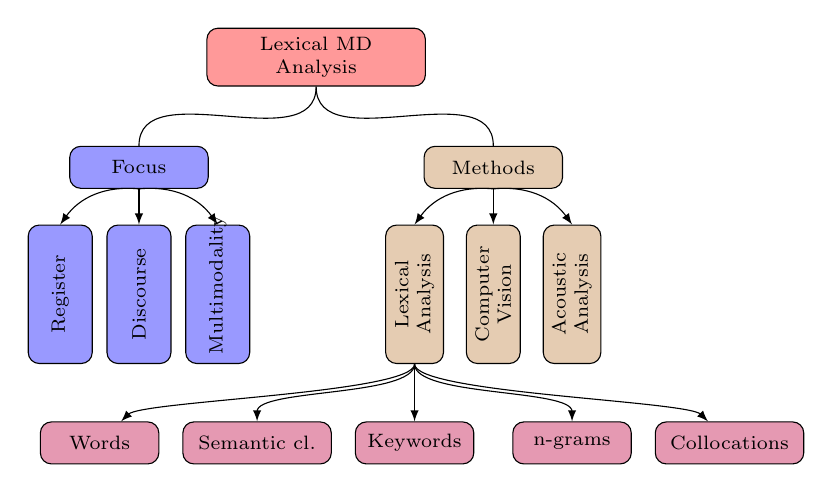
\begin{tikzpicture}
        %\tikzstyle{block} = [rectangle, rounded corners, text=black, text centered, draw=black, minimum height=.3in]
        \tikzstyle{block} = [rectangle, rounded corners, text=black, anchor=north, text centered, draw=black,font=\scriptsize, minimum height=.21in,  text width=.6in]
        \tikzstyle{line} = [-latex,draw=black,line width=.4]
        \tikzstyle{noarrow} = [draw=black,line width=.4]
        \node[block,fill=red!40,text=black, text width=1in] (md) at (9.75,9.5) {Lexical MD Analysis};
        \node[block,fill=blue!40,text=black] (focus) at (7.5,8) {Focus};
        \node[block,fill=brown!40,text=black] (methods) at (12,8) {Methods};
        \node[block,fill=blue!40,text=black, rotate=90, anchor=east, minimum height=.32in] (register) at (6.5,7) {Register};
        \node[block,fill=blue!40,text=black, rotate=90, anchor=east, minimum height=.32in] (discourse) at (7.5,7) {Discourse};
        \node[block,fill=blue!40,text=black, rotate=90, anchor=east, minimum height=.32in] (multimodal) at (8.5,7) {Multimodality};
        \node[block,fill=brown!40,text=black, rotate=90, anchor=east] (lexical) at (11,7) {Lexical Analysis};
        \node[block,fill=brown!40,text=black, rotate=90, anchor=east] (computervision) at (12,7) {Computer Vision};
        \node[block,fill=brown!40,text=black, rotate=90, anchor=east] (acoustic) at (13,7) {Acoustic Analysis};
        \node[block,fill=purple!40,text=black, text width=.5in] (words) at (7,4.5) {Words};
        \node[block,fill=purple!40,text=black, text width=.65in, font=\scriptsize] (semantic) at (9,4.5) {Semantic cl.};
        \node[block,fill=purple!40,text=black, text width=.5in, font=\scriptsize] (keywords) at (11,4.5) {Keywords};
        \node[block,fill=purple!40,text=black, text width=.5in, font=\scriptsize] (bundles) at (13,4.5) {n-grams};
        \node[block,fill=purple!40,text=black, text width=.65in, font=\scriptsize] (collocations) at (15,4.5) {Collocations};
        %\node[block,fill=green!40,text=black, rotate=90, anchor=east, text width=.5in] (words) at (9,5) {\fontsize{6pt}{10pt}\selectfont Words};
        \draw[noarrow] (md) to[in=90,out=270] (focus);
        \draw[noarrow] (md) to[in=90,out=270] (methods);
        \draw[line,-latex] (focus.south) to[bend right] (register.east);
        \draw[line,-latex] (focus.south) to (discourse);
        \draw[line,-latex] (focus.south) to[bend left] (multimodal.east);
        \draw[line,-latex] (methods.south) to[bend right] (lexical.east);
        \draw[line,-latex] (methods.south) to (computervision.east);
        \draw[line,-latex] (methods.south) to[bend left] (acoustic.east);
        \draw[line, looseness=.25] (lexical.west) to[in=45,out=270] (words);
        \draw[line, looseness=.5] (lexical.west) to[in=90,out=270] (semantic);
        \draw[line, looseness=.5] (lexical.west) to[in=90,out=270] (keywords);
        \draw[line, looseness=.5] (lexical.west) to[in=90,out=270] (bundles);
        \draw[line, looseness=.25] (lexical.west) to[in=135,out=270] (collocations);
        %\draw[line,-latex] (apply) to[bend right] node[midway,above]{Some label} (languages.east);
        %\draw[line, densely dashed] (bundapproach) to[in=270,out=90] (bundpattern);
    \end{tikzpicture}
    \caption{Lexical Multi-Dimensional Analysis \citep{berbersardinhaLexicalMultiDimensionalAnalysis2025}}
    \label{fig:lexical_md_analysis}
\end{figure}


\section{Functional Requirements}
\subsection{Corpus Ingestion}
\begin{itemize}
    \item FR-1: Import plain text files, folders, and CSV/TSV with a designated text column;
    \item FR-2: Detect/allow selection of text encoding (UTF-8 default), handle BOM, and report decoding errors;
    \item FR-3: Optional metadata import (e.g., author, source, label) to support grouping and filtering.
\end{itemize}

\subsection{Preprocessing}
\begin{itemize}
    \item FR-4: Tokenise, normalise (case, punctuation policies), and sentence-segment texts;
    \item FR-5: Lemmatise and POS-tag (spaCy models; fallback to NLTK if unavailable);
    \item FR-6: Language selection and multi-language support; warn if models are missing;
    \item FR-7: Stopword management (built-in lists and user-defined additions).
\end{itemize}

\subsection{Feature Extraction}
\begin{itemize}
    \item FR-8: Compute lexical richness metrics (TTR, MTLD, Maas, HDD);
    \item FR-9: Frequency features: word and lemma frequency profiles; function word distributions;
    \item FR-10: POS and POS n-grams; content/function word ratios; lexical sophistication bands;
    \item FR-11: Custom feature plug-ins via a documented Python interface.
\end{itemize}

\subsection{Dimensional Analysis}
\begin{itemize}
    \item FR-12: Build a document-feature matrix (DFM) with configurable weighting (raw, tf-idf, z-scores);
    \item FR-13: Perform dimensionality reduction (PCA) and optional factor analysis (EFA/Varimax);
    \item FR-14: Compute factor loadings, factor scores, and explained variance;
    \item FR-15: Save and load trained models/pipelines for reproducibility.
\end{itemize}

\subsection{Visualisation and GUI}
\begin{itemize}
    \item FR-16: Interactive scatter/biplots of documents in 2D/3D factor space with tooltips and labels;
    \item FR-17: Loading plots, scree plots, and feature contribution charts;
    \item FR-18: Brushing/filtering by metadata, search, and selection for detailed inspection;
    \item FR-19: Theming, layout persistence, and session autosave.
\end{itemize}

\subsection{Export and Reporting}
\begin{itemize}
    \item FR-20: Export factor scores, loadings, and projections to CSV/JSON;
    \item FR-21: Generate PDF/HTML reports with key plots and tables;
    \item FR-22: Export model artifacts (preprocessing config, feature schema, PCA/FA components).
\end{itemize}

\subsection{Automation and Scripting}
\begin{itemize}
    \item FR-23: Batch processing via CLI and/or headless mode;
    \item FR-24: Optional REST API for programmatic access (server mode).
\end{itemize}

\section{Non-Functional Requirements}
\subsection{Performance}
\begin{itemize}
    \item NFR-1: Handle corpora up to 1M tokens on a standard laptop with reasonable latency (\textless 10s for PCA on 10k documents x 1k features, assuming sparse ops);
    \item NFR-2: Incremental processing and caching to avoid recomputation.
\end{itemize}

\subsection{Usability}
\begin{itemize}
    \item NFR-3: Intuitive GUI with sensible defaults; accessible color schemes;
    \item NFR-4: Contextual help and onboarding tips; undo/redo for key actions.
\end{itemize}

\subsection{Reliability and Robustness}
\begin{itemize}
    \item NFR-5: Deterministic pipelines when seeds are fixed; versioned model artifacts;
    \item NFR-6: Error handling with clear diagnostics and recovery suggestions.
\end{itemize}

\subsection{Portability and Compatibility}
\begin{itemize}
    \item NFR-7: Cross-platform support (Windows, macOS, Linux);
    \item NFR-8: Python 3.10+; packaged with virtualenv/Poetry; optional standalone (PyInstaller).
\end{itemize}

\subsection{Security}
\begin{itemize}
    \item NFR-9: Local-only data processing by default; no data leaves the machine;
    \item NFR-10: If server mode enabled, enforce TLS and authentication.
\end{itemize}

\section{System Architecture}
\subsection{Overview}
The system follows a modular, pipeline-oriented architecture separating ingestion, preprocessing, feature extraction, modeling, and presentation layers. A central configuration orchestrates reproducible runs; artifacts are persisted for reuse.

% Optional: include analysis diagrams
% \begin{figure}
    \centering
    %\tikzstyle{block} = [rectangle, rounded corners, text=black, text centered, draw=black, minimum height=.3in]
    %\tikzstyle{block} = [rectangle, rounded corners, text=black, text centered, draw=black,font=\scriptsize, minimum height=.35in, minimum width=.65in]
    \tikzstyle{block} = [rectangle, rounded corners, text=black, text centered, draw=black,font=\scriptsize, minimum width=1.6in, minimum height=.2in]
    \tikzstyle{line} = [-latex,draw=black,line width=.5, densely dotted]
    \tikzstyle{line2} = [latex-latex,draw=black,line width=.4, densely dashed]
    \tikzstyle{line3} = [-latex,draw=black,line width=.4, densely dotted]
    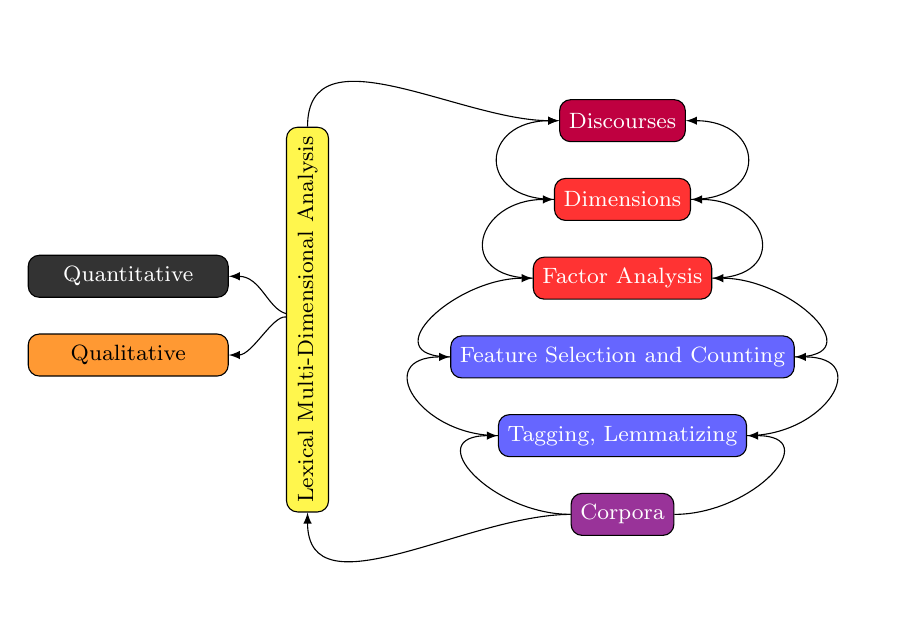
\begin{tikzpicture}
        \node[block,fill=purple!100,text=white, anchor=north] (regul) at (10,10) {Discourses};
        \node[block,fill=red!80,text=white, anchor=north] (recur) at (10,9) {Dimensions};
        \node[block,fill=red!80,text=white, anchor=north] (cooc) at (10,8) {Factor Analysis};
        \node[block,fill=blue!60,text=white, anchor=north] (stats) at (10,7) {Feature Selection and Counting};
        \node[block,fill=blue!60,text=white, anchor=north] (bottomup) at (10,6) {Tagging, Lemmatizing};
        \node[block,fill=violet!80,text=white, anchor=north] (corpora) at (10,5) {Corpora};
        \node[block, fill=yellow!70, text=black, rotate=90, minimum width=1.6in] (compute) at (6,7.2) {Lexical Multi-Dimensional Analysis};
        \node[block,fill=black!80,text=white, anchor=east, minimum width=1in] (quant) at (5,7.75) {Quantitative};
        \node[block,fill=orange!80,text=black, anchor=east, minimum width=1in] (qual) at (5,6.75) {Qualitative};
        %\node[block, fill=purple!40, text=white, rotate=90, minimum width=1.6in] (mda) at (14,7.2) {Multi-Dimensional Analysis};
        %\node[block,fill=purple!10,text=black,text width=.75in, anchor=north, dashed] (underlying) at (10,9.75) {Underlying dimensions};
        \draw[line] (corpora.east) .. controls +(1,0) and +(1,0) .. (bottomup.east);
        \draw[line] (bottomup.east) .. controls +(1,0) and +(1,0) .. (stats.east);
        \draw[line] (stats.east) .. controls +(1,0) and +(1,0) .. (cooc.east);
        \draw[line] (cooc.east) .. controls +(1,0) and +(1,0) .. (recur.east);
        \draw[line] (recur.east) .. controls +(1,0) and +(1,0) .. (regul.east);
        \draw[line] (corpora.west) .. controls +(-1,0) and +(-1,0) .. (bottomup.west);
        \draw[line] (bottomup.west) .. controls +(-1,0) and +(-1,0) .. (stats.west);
        \draw[line] (stats.west) .. controls +(-1,0) and +(-1,0) .. (cooc.west);
        \draw[line] (cooc.west) .. controls +(-1,0) and +(-1,0) .. (recur.west);
        \draw[line] (recur.west) .. controls +(-1,0) and +(-1,0) .. (regul.west);
        \draw[line] (corpora) to[out=180, in=270] (compute.west);
        \draw[line] (compute.east) to[out=90, in=180] (regul);
        \draw[line] (compute) to [out=125, in=0] (quant);
        \draw[line] (compute) to [out=125, in=0] (qual);
        %\draw[line2] (cognition) to [in=270,out=270] (society);
        %\draw[line2] (cognition) .. controls +(0,-1) and +(0,-1) .. (society);
    \end{tikzpicture}
    %\footnotetext{Mostly.}
    \caption{Lexical Multi-Dimensional Analysis 1 \citep{berbersardinhaLexicalMultiDimensionalAnalysis2025}}
    \label{fig:lexical_md_analysis1}
\end{figure}

% \begin{figure}
    \centering
    %\tikzstyle{block} = [rectangle, rounded corners, text=black, text centered, draw=black, minimum height=.3in]
    %\tikzstyle{block} = [rectangle, rounded corners, text=black, text centered, draw=black,font=\scriptsize, minimum height=.35in, minimum width=.65in]
    \tikzstyle{block} = [rectangle, rounded corners, text=black, text centered, draw=black,font=\scriptsize, minimum width=1.2in, minimum height=.2in]
    \tikzstyle{line} = [-latex,draw=black,line width=.5, densely dotted]
    \tikzstyle{line2} = [latex-latex,draw=black,line width=.4, densely dashed]
    \tikzstyle{line3} = [-latex,draw=black,line width=.4, densely dotted]
    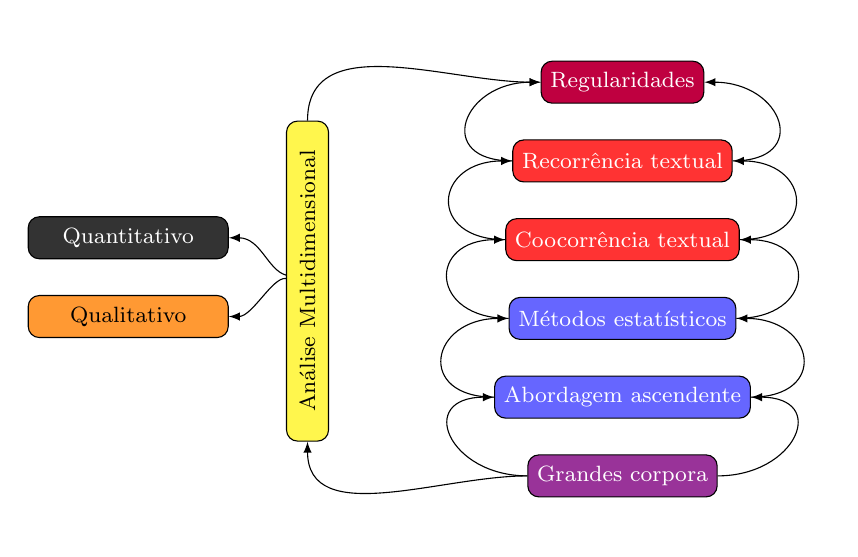
\begin{tikzpicture}
        \node[block,fill=purple!100,text=white, anchor=north] (regul) at (10,10) {Regularidades};
        \node[block,fill=red!80,text=white, anchor=north] (recur) at (10,9) {Recorrência textual};
        \node[block,fill=red!80,text=white, anchor=north] (cooc) at (10,8) {Coocorrência textual};
        \node[block,fill=blue!60,text=white, anchor=north] (stats) at (10,7) {Métodos estatísticos};
        \node[block,fill=blue!60,text=white, anchor=north] (bottomup) at (10,6) {Abordagem ascendente};
        \node[block,fill=violet!80,text=white, anchor=north] (corpora) at (10,5) {Grandes corpora};
        \node[block, fill=yellow!70, text=black, rotate=90, minimum width=1.6in] (compute) at (6,7.2) {Análise Multidimensional};
        \node[block,fill=black!80,text=white, anchor=east, minimum width=1in] (quant) at (5,7.75) {Quantitativo};
        \node[block,fill=orange!80,text=black, anchor=east, minimum width=1in] (qual) at (5,6.75) {Qualitativo};
        %\node[block, fill=purple!40, text=white, rotate=90, minimum width=1.6in] (mda) at (14,7.2) {Multi-Dimensional Analysis};
        %\node[block,fill=purple!10,text=black,text width=.75in, anchor=north, dashed] (underlying) at (10,9.75) {Underlying dimensions};
        \draw[line] (corpora.east) .. controls +(1,0) and +(1,0) .. (bottomup.east);
        \draw[line] (bottomup.east) .. controls +(1,0) and +(1,0) .. (stats.east);
        \draw[line] (stats.east) .. controls +(1,0) and +(1,0) .. (cooc.east);
        \draw[line] (cooc.east) .. controls +(1,0) and +(1,0) .. (recur.east);
        \draw[line] (recur.east) .. controls +(1,0) and +(1,0) .. (regul.east);
        \draw[line] (corpora.west) .. controls +(-1,0) and +(-1,0) .. (bottomup.west);
        \draw[line] (bottomup.west) .. controls +(-1,0) and +(-1,0) .. (stats.west);
        \draw[line] (stats.west) .. controls +(-1,0) and +(-1,0) .. (cooc.west);
        \draw[line] (cooc.west) .. controls +(-1,0) and +(-1,0) .. (recur.west);
        \draw[line] (recur.west) .. controls +(-1,0) and +(-1,0) .. (regul.west);
        \draw[line] (corpora) to[out=180, in=270] (compute.west);
        \draw[line] (compute.east) to[out=90, in=180] (regul);
        \draw[line] (compute) to [out=125, in=0] (quant);
        \draw[line] (compute) to [out=125, in=0] (qual);
        %\draw[line2] (cognition) to [in=270,out=270] (society);
        %\draw[line2] (cognition) .. controls +(0,-1) and +(0,-1) .. (society);
    \end{tikzpicture}
    %\footnotetext{Mostly.}
    \caption{Lexical Multi-Dimensional Analysis 2 \citep{berbersardinhaLexicalMultiDimensionalAnalysis2025}}
    \label{fig:lexical_md_analysis2}
\end{figure}

% \begin{figure}
    \centering
    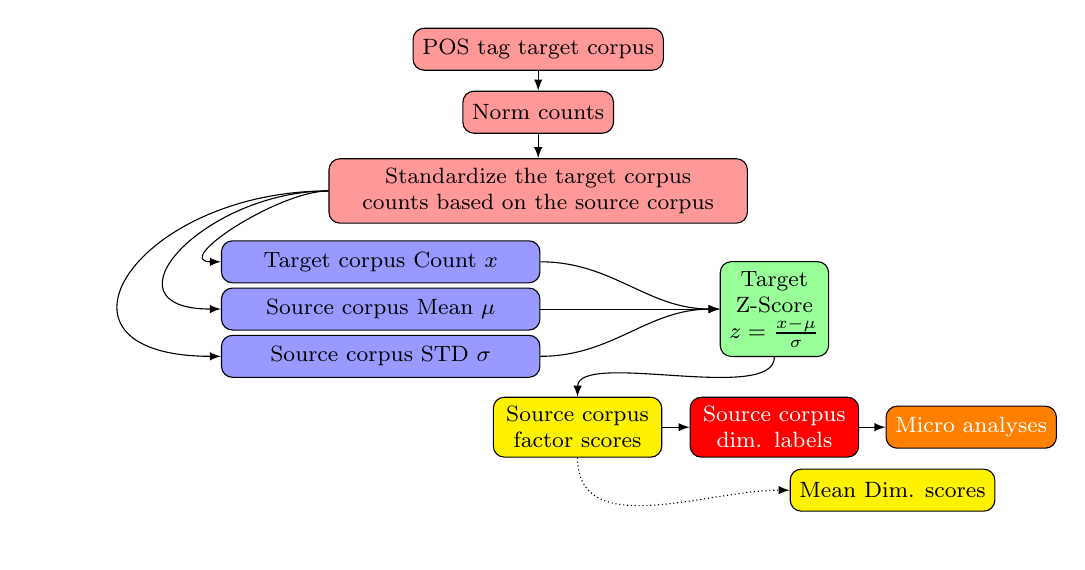
\begin{tikzpicture}
        %\tikzstyle{block} = [rectangle, rounded corners, text=black, text centered, draw=black, minimum height=.3in]
        \tikzstyle{block} = [rectangle, rounded corners, text=black, text centered, draw=black,font=\footnotesize, minimum height=.21in]
        \tikzstyle{line} = [-latex,draw=black,line width=.4]
        \node[block,fill=red!40,text=black] (tag) at (5,3) {POS tag target corpus};
        \node[block,fill=red!40,text=black] (norm) at (5,2.2) {Norm counts};
        \node[block,fill=red!40,text=black, text width=2in] (score1) at (5,1.2) {Standardize the target corpus counts based on the source corpus};
        \node[block,fill=blue!40,text=black, text width=1.5in] (count) at (3,.3) {Target corpus Count $x$};
        \node[block,fill=blue!40,text=black, text width=1.5in] (mean) at (3,-.3) {Source corpus Mean $\mu$};
        \node[block,fill=blue!40,text=black, text width=1.5in] (std) at (3,-.9) {Source corpus STD $\sigma$};
        %\node[block,fill=blue!40,text=black] (comm) at (1,-.2) {Commun.};
        \node[block,fill=green!40,text=black,align=center] (zscore) at (8,-.3) {Target \\ Z-Score \\ \( z = \frac{{x - \mu}}{{\sigma}} \)};
        %\node[block,fill=green!40,text=black] (load) at (7,-.2) {Drop weak loadings};
        %\node[block,fill=green!40,text=black] (standard) at (7,-1) {Standardize counts};
        \node[block,fill=yellow,text=black, text width=.75in] (scores) at (5.5,-1.8) {Source corpus factor scores};
        \node[block,fill=red,text=white, text width=.75in] (labels) at (8,-1.8) {Source corpus dim. labels};
        \node[block,fill=orange,text=white] (analyze) at (10.5,-1.8) {Micro analyses};
        \node[block,fill=yellow,text=black] (dimscores) at (9.5,-2.6) {Mean Dim. scores};
        \draw[line] (tag) to (norm);
        \draw[line] (norm) to (score1);
        \draw[line, densely dotted] (scores) to[in=180,out=270] (dimscores);
        %\draw[line,densely dashed] (standard) to (labels);
        %\draw[line,loosely dashed] (standard) to (labels);
        \draw[line] (score1) to[in=180,out=180,looseness=1] (count);
        \draw[line] (score1) to[in=180,out=180,looseness=2] (mean);
        \draw[line] (score1) to[in=180,out=180,looseness=2.5] (std);
        \draw[line] (count) to[in=180,out=0] (zscore);
        \draw[line] (mean) to[in=180,out=0] (zscore);
        \draw[line] (std) to[in=180,out=0] (zscore);
        \draw[line] (zscore) to[in=90,out=270,looseness=.6] (scores);
        \draw[line] (scores) to[in=180,out=0] (labels);
        \draw[line] (labels) to (analyze);
        %\draw[line] (zscore) to[out=180,in=90] (0,-1.5) to[out=270,in=180] (scores);
    \end{tikzpicture}
    \caption{Additive Multi-Dimensional Analysis \citep{biberVariationEnglishMultiDimensional2001, berbersardinhaAddingRegistersPrevious2019}}
    \label{fig:additive_md_analysis}
\end{figure}


\subsection{Components}
\paragraph{GUI Layer}
Desktop GUI (PySide6/PyQt) for user workflows: project management, corpus loading, configuration, visualisation, and export.

\paragraph{Controller / Orchestration}
Coordinates pipeline stages, manages state, triggers incremental recomputation when inputs change, and logs provenance.

\paragraph{Preprocessing Service}
Language detection, sentence segmentation, tokenisation, lemmatisation, POS tagging, stopword filtering; caches normalised representations.

\paragraph{Feature Service}
Computes metrics and vectorises documents into a DFM with configurable normalisation and weighting; supports plug-ins.

\paragraph{Modeling Service}
Performs PCA/EFA, computes loadings and scores, applies rotations (e.g., Varimax/Promax), and persists models.

\paragraph{Visualisation Service}
Generates interactive plots (2D/3D scatter, biplots, scree, loadings) and data tables; supports selections and linked views.

\paragraph{Persistence Layer}
Stores corpora metadata, preprocessed artifacts, features, and models (e.g., SQLite for metadata, parquet/npz for matrices, joblib for models).

\paragraph{API Layer (Optional)}
FastAPI-based REST endpoints for batch/remote processing in server mode.

\subsection{Data Flow}
\begin{enumerate}
    \item Import corpus $\rightarrow$ normalise text $\rightarrow$ linguistic annotation.
    \item Extract features $\rightarrow$ construct DFM $\rightarrow$ apply weighting/normalisation.
    \item Fit PCA/EFA $\rightarrow$ compute scores/loadings $\rightarrow$ store artifacts.
    \item Visualise and interact $\rightarrow$ export results and reports.
\end{enumerate}

\section{Technology Stack}
\begin{itemize}
    \item Language: Python 3.11 (or 3.10+);
    \item GUI: PySide6 or PyQt6; alternative: Qt for Python widgets + matplotlib/plotly;
    \item NLP: spaCy (core models: \texttt{en\_core\_web\_sm/md/lg}), NLTK (fallback, resources), langdetect/fastText for language ID;
    \item Data: pandas, numpy, scipy (sparse matrices), scikit-learn for PCA, factor analyzers (\texttt{factor\_analyzer}) for EFA/rotations;
    \item Visualisation: matplotlib, seaborn, plotly; pyqtgraph for fast interactive plots;
    \item Persistence: SQLite (metadata), parquet/CSV (tables), npz (sparse matrices), joblib/pickle (models), YAML/TOML (config);
    \item Packaging: Poetry or pip-tools; PyInstaller for desktop bundle; Docker for server mode;
    \item Testing: pytest, hypothesis for property-based testing, tox/\texttt{nox} for matrix runs;
    \item CI/CD: GitHub Actions or GitLab CI for tests, linting (ruff, black), and packaging.
\end{itemize}

\section{Interfaces and APIs}
\subsection{Python Module Interfaces}
\begin{itemize}
    \item \textbf{Preprocessor}: \texttt{process(corpus, config) $\rightarrow$ annotations};
    \item \textbf{FeatureExtractor}: \texttt{fit\_transform(annotations) $\rightarrow$ DFM}; \texttt{transform(...)};
    \item \textbf{Modeler}: \texttt{fit(DFM) $\rightarrow$ model}; \texttt{transform(DFM) $\rightarrow$ scores};
    \item \textbf{Visualiser}: \texttt{plots(scores, loadings, metadata)};
    \item \textbf{Persistence}: \texttt{save\_artifact(obj, kind)} and \texttt{load\_artifact(kind)}.
\end{itemize}

\subsection{Plug-in Interface}
Third-party feature extractors implement \texttt{IFeaturePlugin}:
\begin{itemize}
    \item \texttt{schema()} returns feature names and dtypes;
    \item \texttt{compute(doc)} yields a sparse/compact feature vector;
    \item Registration via entry points or a plugins folder.
\end{itemize}

\subsection{CLI}
\begin{verbatim}
lmda run --config config.yaml --input corpus/ --output artifacts/
lmda visualise --project my_project.lmda
\end{verbatim}

\subsection{Optional REST API (FastAPI)}
\begin{itemize}
    \item POST /v1/projects: create project
    \item POST /v1/projects/{id}/ingest: upload texts/metadata
    \item POST /v1/projects/{id}/run: execute pipeline
    \item GET /v1/projects/{id}/scores: factor scores
    \item GET /v1/projects/{id}/loadings: factor loadings
    \item GET /v1/projects/{id}/report: PDF/HTML report
\end{itemize}

\section{Security and Privacy Considerations}
\subsection{Data Protection}
\begin{itemize}
    \item Local-first processing; no external calls by default;
    \item Optional at-rest encryption for project files; secure temp directories;
    \item Configurable redaction of personally identifiable information (PII) in exports.
\end{itemize}

\subsection{Access Control (Server Mode)}
\begin{itemize}
    \item Authentication (OAuth2/JWT) and role-based access control (RBAC);
    \item TLS enforcement; secure headers and CSRF protections for Web GUI (if used).
\end{itemize}

\subsection{Supply Chain}
\begin{itemize}
    \item Pin dependencies; verify wheels; use vulnerability scanning (pip-audit, Safety);
    \item Sandboxed plug-ins with permission checks.
\end{itemize}

\section{Risks and Mitigations}
\begin{itemize}
    \item \textbf{R1: Model interpretability} — Factors may be hard to interpret. \\
          \emph{Mitigation}: Offer rotations, feature contribution charts, and glossary tooltips.
    \item \textbf{R2: Performance on large corpora} — High memory/CPU usage. \\
          \emph{Mitigation}: Sparse structures, incremental processing, caching, chunked I/O.
    \item \textbf{R3: NLP model availability} — spaCy models not installed. \\
          \emph{Mitigation}: Guided download, fallback tokenisers, graceful degradation.
    \item \textbf{R4: Data privacy} — Sensitive texts accidentally exported. \\
          \emph{Mitigation}: Local-first defaults, explicit consent prompts, export redaction.
    \item \textbf{R5: Cross-platform GUI quirks} — Rendering differences. \\
          \emph{Mitigation}: UI testing matrix, use of Qt styles, theming validation.
    \item \textbf{R6: Reproducibility drift} — Version changes affect outputs. \\
          \emph{Mitigation}: Lockfiles, artifact versioning, seeds, environment capture.
\end{itemize}

\section{Timeline and Milestones}
\begin{enumerate}
    \item \textbf{Week 1--2: Foundations} \\
          Project scaffolding, env setup, CI/CD, basic data model, configuration schema;
    \item \textbf{Week 3--4: Preprocessing} \\
          Language detection, tokenisation, lemmatisation, POS tagging; caching;
    \item \textbf{Week 5--6: Features} \\
          Core lexical metrics, function word profiles, POS n-grams; plug-in API;
    \item \textbf{Week 7--8: Modeling} \\
          PCA/EFA pipeline, rotations, persistence; basic CLI;
    \item \textbf{Week 9--10: GUI v1} \\
          Data loading, configuration panels, 2D scatter, scree and loadings plots;
    \item \textbf{Week 11--12: Reporting \& Export} \\
          CSV/JSON exports, PDF/HTML reports; theming and preferences;
    \item \textbf{Week 13--14: Hardening} \\
          Performance tuning, testing, error handling, documentation;
    \item \textbf{Week 15+: Optional Server Mode} \\
          FastAPI endpoints, auth/TLS, Docker packaging.
\end{enumerate}
